\section{Background}\label{sec:background}

Consider the strictly convex\footnote{The case when $Q \succeq 0$ is treated in a later section.} quadratic program:
\begin{equation}\label{eq:qp}
\begin{aligned}
\min_{x \in \R^n} \quad & f(x) = \tfrac{1}{2}x^\top Q x + g^\top x \\
\text{subject to} \quad & a_i^\top x \leq b_i, \quad i = 1,\ldots,m,
\end{aligned}
\end{equation}
where $Q \in \R^{n \times n}$ is symmetric positive definite, $g \in \R^n$, and each constraint $(a_i, b_i) \in \R^n \times \R$ with $a_i \neq 0$. 

\begin{definition}\label{def:polytope}
The feasible region is the polytope
\begin{equation}
\mathcal{P} = \{x \in \R^n : Ax \leq b\},
\end{equation}
where $A = [a_1, \ldots, a_m]^\top \in \R^{m \times n}$ and $b = [b_1, \ldots, b_m]^\top \in \R^m$. Throughout, we assume $\mathcal{P}$ is non-empty, bounded, and has non-empty interior.
\end{definition}

\begin{definition}\label{def:xbar}
Since $Q \succ 0$, the objective $f$ has a unique global minimizer
\begin{equation}
\bar{x} = -Q^{-1}g,
\end{equation}
\end{definition}

The constrained minimizer $x^\star$ to \eqref{eq:qp} satisfies the Karush--Kuhn--Tucker (KKT) conditions: $ \exists \lambda^\star \in \R^m$ such that,
\begin{subequations}
\begin{align}
Qx^\star + g - A^\top \lambda^\star &= 0, \label{eq:kkt_stationarity}\\
Ax^\star &\leq b, \label{eq:kkt_primal}\\
\lambda^\star &\geq 0, \label{eq:kkt_dual}\\
\lambda_i^\star(a_i^\top x^\star - b_i) &= 0, \quad i=1,\ldots,m. \label{eq:kkt_complementarity}
\end{align}
\end{subequations}

The \emph{active set} at $x^\star$ is $\mathcal{A}^\star = \{i : a_i^\top x^\star = b_i\}$. Active-set methods solve \eqref{eq:qp} by iteratively adjusting the active set, solving a sequence of equality-constrained subproblems until optimality is reached.


\begin{definition}\label{def:face}
A \emph{face} of $\mathcal{P}$ is a set of the form
\begin{equation}
F = \{x \in \mathcal{P} : a_i^\top x = b_i \text{ for all } i \in \mathcal{I}\}
\end{equation}
for some index set $\mathcal{I} \subseteq \{1,\ldots,m\}$. The \emph{dimension} of $F$ is $\dim(F) = \dim(\aff(F))$. 
\begin{itemize}
    \item A \emph{facet} (codimension-1 face) satisfies $\dim(F) = n-1$.
    \item A \emph{ridge} (codimension-2 face) satisfies $\dim(F) = n-2$.
    \item A \emph{vertex} (0-dimensional face) is a point.
\end{itemize}
The \emph{relative interior} of $F$, denoted $\relint(F)$, consists of points in $F$ that are not in any proper subface of $F$.
\end{definition}

\begin{remark}\label{rem:vertex}
    From Definition \ref{def:face}, a vertex $v \in \mathcal{P}$ is necessarily such that the set of vectors $a_i : a_i^\top v = b_i$ span $\mathbb{R}^n$. This clearly has computational application when one is interested in finding a vertex (enumerating vertices) of $\mathcal{P}$.
\end{remark}

\begin{definition}\label{def:adjacent}
Two distinct faces $F_1, F_2$ of $\mathcal{P}$ are \emph{adjacent} if $F_1 \cap F_2$ is a face of dimension $\min\{\dim(F_1), \dim(F_2)\} - 1$. Equivalently, two facets are adjacent if they share a common ridge.
\end{definition}

\begin{example}\label{ex:adjacency}
In $\R^2$, facets are edges, and two edges are adjacent if they share a vertex. In $\R^3$, facets are polygonal faces, and two faces are adjacent if they share an edge. 
\end{example}

\begin{definition}\label{def:normal_cone}
Let $x \in \mathcal{P}$.  
The \emph{normal cone} to $\mathcal{P}$ at $x$ is defined as
\begin{equation}
N_{\mathcal{P}}(x)
=
\{\, y \in \mathbb{R}^n \;:\; \langle y, z - x \rangle \le 0 \;\; \forall z \in \mathcal{P} \,\}.
\end{equation}
If $x$ lies in the relative interior of a face $F$, then 
\begin{equation}
N_{\mathcal{P}}(x) = \operatorname{cone}\{ a_i : i \in \mathcal{A}(x) \}
\end{equation}
and is constant over $\relint(F)$.
\end{definition}

Some particular classes of polytopes, namely \textit{well conditioned} polytopes are of special interest. The following two non-standard but intuitive definitions establish their properties.

\begin{definition}
The directional width of $\mathcal P$
in direction $\nu$ is defined as
\[
w_{\mathcal P}(\nu)
\;:=\;
\max_{x \in \mathcal P} \langle \nu, x \rangle
\;-\;
\min_{x \in \mathcal P} \langle \nu, x \rangle.
\]
\end{definition}
\begin{definition}\label{def:well_behaved}
A bounded convex polytope $\mathcal P \subset \mathbb R^n$ is said to be
$\kappa$-well-conditioned if there exists a constant $\kappa > 0$ such that
\[
w_{\mathcal P}(\nu) \;\le\; \kappa
\quad \text{for all } \nu \in \mathbb S^{n-1}.
\]
\end{definition}

A central construction of this paper is the notion of a \emph{good vertex} relative to an exterior point.

\begin{definition}\label{def:good_vertex}
Let $\bar{x} \notin \mathcal{P}$. A vertex $v$ of $\mathcal{P}$ is \emph{good} (with respect to $\bar{x}$) if the ray from $v$ toward $\bar{x}$ enters the interior of $\mathcal{P}$ for small positive $t$:
\begin{equation}
\exists \epsilon > 0 : \{v + t(\bar{x} - v) : 0 < t < \epsilon\} \subset \relint(\mathcal{P}).
\end{equation}
Equivalently, for all constraints $i$ active at $v$ (i.e., $a_i^\top v = b_i$), we have
\begin{equation}\label{eq:good_vertex_condition}
a_i^\top(\bar{x} - v) < 0.
\end{equation}
Equivalently, $\bar{x} - v$ lies in the interior of the tangent cone 
$T_v\mathcal{P}$
\end{definition}

\begin{remark}\label{rem:good_intuition}
A vertex $v$ is good if it \enquote{sees} $\bar{x}$ through the interior of $\mathcal{P}$. The condition \eqref{eq:good_vertex_condition} requires that all active constraint normals point \emph{away} from the direction toward $\bar{x}$. In $\R^2$ for instance, a convex polygon has exactly two edges meeting at each vertex, forming an interior angle. A vertex is good if $\bar{x}$ lies within the cone formed by extending these two edges. Unless $\bar{x} \in \mathcal{P}$, not all vertices can be good simultaneously.
\end{remark}

The above definition and discussion lead us to state our main assumption for this manuscript.

\begin{assumption}\label{as:non_empty_vgood}
We assume there exists at least one vertex $v \in P$ such that the ray $v + t(\bar x - v)$ enters $\mathrm{int}(P)$ for all sufficiently small $t>0$. The set of such vertices is denoted $V_\text{good}$.
\end{assumption}

Note that Assumption~\ref{as:non_empty_vgood} is needed since the existence of a good vertex is not guaranteed for arbitrary convex polytopes.
In particular, even in $\mathbb{R}^2$, there exist polytopes and exterior points
for which no vertex sees $\bar x$ through the interior.
Figure~1 illustrates these aspects. In cases where no good vertex exits, one could still employ the usual centroid (or internal point) fallback routines as will be discussed in Section~\ref{sec:algorithms}.




\begin{figure}[h!]
\centering
\fbox{
\begin{minipage}{0.95\textwidth}
\centering
\begin{subfigure}[b]{0.3\textwidth}
\centering
\begin{tikzpicture}[scale=1.1]
\coordinate (v1) at (1,0); \coordinate (v2) at (2,0.5);
\coordinate (v3) at (2.5,1.5); \coordinate (v4) at (2,2.5);
\coordinate (v5) at (1,3); \coordinate (v6) at (0,2.5);
\coordinate (v7) at (-0.5,1.5); \coordinate (v8) at (0,0.5);
\draw[thick] (v1) -- (v2) -- (v3) -- (v4) -- (v5) -- (v6) -- (v7) -- (v8) -- cycle;
\fill[blue!10] (v1) -- (v2) -- (v3) -- (v4) -- (v5) -- (v6) -- (v7) -- (v8) -- cycle;
\coordinate (xbar) at (3.5,1.5); \filldraw[red] (xbar) circle (2pt); \node[above right] at (xbar) {$\bar{x}$};
\foreach \v in {v6,v7,v8} {\filldraw[green!70!black] (\v) circle (2.5pt);}
\draw[dashed,->,green!70!black] (v6) -- ($(v6)!0.9!(xbar)$);
\draw[dashed,->,green!70!black] (v7) -- ($(v7)!0.9!(xbar)$);
\draw[dashed,->,green!70!black] (v8) -- ($(v8)!0.9!(xbar)$);
\end{tikzpicture}
\caption{Several good vertices}
\end{subfigure}
\hfill
\begin{subfigure}[b]{0.3\textwidth}
\centering
\begin{tikzpicture}[scale=3.5,tdplot_main_coords]
\tdplotsetmaincoords{60}{120}

\coordinate (v1) at (0,0,0); 
\coordinate (v2) at (1,0,0);
\coordinate (v3) at (0.5,0.866,0);
\coordinate (v4) at (0.5,0.289,0.816); 

\draw[thick] (v1) -- (v2) -- (v3) -- cycle;
\draw[thick] (v1) -- (v4); \draw[thick] (v2) -- (v4); \draw[thick] (v3) -- (v4);

\fill[blue!10,opacity=0.5] (v1) -- (v2) -- (v3) -- cycle;
\fill[blue!10,opacity=0.5] (v1) -- (v2) -- (v4) -- cycle;
\fill[blue!10,opacity=0.5] (v2) -- (v3) -- (v4) -- cycle;
\fill[blue!10,opacity=0.5] (v3) -- (v1) -- (v4) -- cycle;

\coordinate (xbar) at (1.4,0.5,0.8); \filldraw[red] (xbar) circle (0.8pt); \node[above] at (xbar) {$\bar{x}$};

\filldraw[green!70!black] (v1) circle (0.8pt); 
%\node[left] at (v1) {$v_{\text{good}}$};
\draw[dashed,->,green!70!black] (v1) -- ($(v1)!0.9!(xbar)$);

% % Other vertex labels
\end{tikzpicture}
\caption{Single good vertex}
\end{subfigure}
\begin{subfigure}[b]{0.3\textwidth}
\centering
\begin{tikzpicture}[scale=1.5]

% --- House polytope vertices ---
\coordinate (v1) at (0,0);
\coordinate (v2) at (2,0);
\coordinate (v4) at (1.2,0.5);  % small roof peak
\coordinate (v5) at (0.8,0.5);

\draw[thick]
  (v1) -- (v2)  -- (v4) -- (v5) -- cycle;
\fill[blue!10]
  (v1) -- (v2) --  (v4) -- (v5) -- cycle;

\coordinate (xbar) at (1.0,2.1);
\filldraw[red] (xbar) circle (2pt);
\node[above right] at (xbar) {$\bar{x}$};

\foreach \v in {v1, v2, v4,v5}
  \draw[dashed,->,gray] (\v) -- ($( \v)!0.9!(xbar)$);
\end{tikzpicture}
\caption{No good vertex exists}
\end{subfigure}

\caption{\emph{Good vertices} in 2D and 3D. Green vertices are good; red point is the exterior $\bar{x}$.}
\end{minipage}
} % end fbox
\end{figure}


\section{Main Results}\label{sec:main_results}

We now state our main claims and present supporting technical results. Throughout the sequel, we use for the M-weighted norm $\norm{x} = \sqrt{x^\top M x}$, with symmetric $M \succ 0$. Similarly, inner products are taken with respect to $M$.

\begin{theorem}
\label{thm:main}
Let $\mathcal P \subset \mathbb R^n$ be a bounded convex polytope with nonempty interior.
Let $\bar x \notin \mathcal P$ and denote
\begin{align}\label{eq:xhat_and_nu}
\hat x = \Proj_{\mathcal P}^M(\bar x), \qquad
\nu = \frac{M(\bar x - \hat x)}{\|M(\bar x - \hat x)\|}.
\end{align}
Assume that the normal cone $N_{\mathcal P}(\hat x)$ has nonempty interior. Further Suppose Assumption~\ref{as:non_empty_vgood} holds, and 
let $v^\star \in V_
\text{good}$ be a farthest good vertex with respect to $\bar x$, and define the ray
$
r(t) = v^\star + t(\bar x - v^\star), \quad t \ge 0.
$
Let $F_0$ be the face through which $r(t)$ exits $\mathcal P$. Let $\mathcal{F}_{\min}$ be the set of faces closest to $\bar{x}$
\begin{equation}\label{eq:closest_faces}
\mathcal{F}_{\min} = \left\{F : \dist(\bar{x}, F) = \min_{F' \text{ face}} \dist(\bar{x}, F')\right\},
\end{equation}
where $\dist(\bar{x}, F) = \inf_{x \in F} \norm{x - \bar{x}}$.
Then, if
\begin{align}\label{eq:L_bound}
L := \|\bar x - \hat x\| \ge w_{\mathcal P}(\nu),
\end{align}
the exit face $F_0$ satisfies:
\begin{enumerate}
    \item Either $F_0$ is a closest face to $\bar x$, or
    \item $F_0$ is adjacent to a closest face.
\end{enumerate}
\end{theorem}

% \begin{remark}
% As $L$ increases, the quadratic term in the $M$-weighted distance becomes negligible, 
% and the farthest good vertex $v^\star$ aligns with the maximizer of $\langle \nu, v \rangle$ 
% over all vertices $v \in \mathcal P$. 
% \end{remark}

\begin{remark}\label{rem:good_vertex_is_hard}
Theorem~\ref{thm:main} hinges on finding $v^\star = \argmax_{v \in V_{\text{good}}} \norm{v - \bar{x}}$. This could be intractable for general polytopes (requires
    enumerating vertices of $\mathcal{P}$ up to $\binom{m}{n}$ vertices in the worst case, and solving a maximization subject to the ray being in the interior). For some classes of polytopes, as we will see one could find either exact solutions (e.g., box-like polytopes) or efficient heuristics (e.g., greedy constraints selections).  
\end{remark}

The farthest good vertex $v^\star$, when viewed as a possible intialization point, and unlike centroid-based initialization (which depends on the distribution of vertices and may exit the polytope through geometrically irrelevant faces), is an extremal point defined by the directional width $w_{\mathcal P}(\nu)$. The resulting ray follows the maximal chord of $\mathcal P$ in direction $\nu$, is invariant to redundant vertices, and preferentially intersects a face close to the optimal active set.


It is important to stress that Theorem~\ref{thm:main} only requires boundedness, convexity, and non-empty interior, thus applying to a large class of convex polytopes typically encountered in quadratic programming. However, to prove it, we need to establish intermediate and helpful technical results. 

\subsection{Farthest Good Vertex}
While calculating exact distances is computationally expensive for generic norms, the separation geometry provides a linear proxy that could be made exact (up to bounds).
\begin{lemma}\label{lem:separation_unified}
There exist a unit vector $\nu \in \R^n$, unique (up to scaling), and $c \in \R$ such that
\begin{equation}\label{eq:separation_unified}
\inner{\nu}{\bar{x}} > c \quad \text{and} \quad \inner{\nu}{x} \leq c \quad \forall x \in \mathcal{P}.
\end{equation}
\end{lemma}

\begin{proof}
By the separating hyperplane theorem for convex sets \cite{conv_book_1}, there exists a hyperplane strictly separating $\bar{x}$ from $\mathcal{P}$. The normal $\nu$ to this hyperplane is determined by the projection $\hat{x}$ and the metric $M$. The projection is characterized by
\begin{equation*}
\bar{x} - \hat{x} = M^{-1} \sum_{i \in \mathcal{A}(\hat{x})} \lambda_i a_i,
\end{equation*}
where $\mathcal{A}(\hat{x}) = \{i : a_i^\top \hat{x} = b_i\}$ are the active constraints at $\hat{x}$, and $\lambda_i \geq 0$ are the Lagrange multipliers. Thus, $\nu \propto M(\bar{x} - \hat{x})$ is a non-negative combination of constraint normals, pointing outward from $\mathcal{P}$ toward $\bar{x}$.
\end{proof}



\begin{lemma}\label{lem:farthest_exact}
The farthest good vertex $v^\star = \argmax_{v \in V_{\text{good}}} \|v - \bar{x}\|$ satisfies:
\begin{equation}
v^\star \in \argmin_{v \in V_{\text{good}}} \left[ \|v - \hat{x}\|^2 - 2L\langle \nu, v - \hat{x}\rangle \right].
\end{equation}
Moreover, if there exists a good vertex $v_0$ such that
\begin{equation}\label{eq:sufficient_condition}
\langle \nu, v_0 - \hat{x}\rangle < \min_{v \in V_{\text{good}} \setminus \{v_0\}} \langle \nu, v - \hat{x}\rangle - \frac{D^2}{2L},
\end{equation}
where $D = \diam(\mathcal{P})$, then $v^\star = v_0$.
In particular, if $L \geq D^2/\epsilon$ for any desired precision $\epsilon > 0$, then
\begin{equation}
v^\star = \argmin_{v \in V_{\text{good}}} \langle \nu, v \rangle.
\end{equation}
\end{lemma}

\begin{proof}
By definition, $\bar{x} = \hat{x} + L\nu$ and one can write
\begin{align*}
\norm{v - \bar{x}}^2 &= \norm{v - (\hat{x} + L\nu)}^2 \\
&= \norm{(v - \hat{x}) - L\nu}^2 \\
&= \norm{v - \hat{x}}^2 - 2\inner{v - \hat{x}}{L\nu} + \norm{L\nu}^2.
\end{align*}

Dropping the constant $L^2$, maximizing $\|v - \bar{x}\|^2$ is equivalent to maximizing $
h(v) := \|v - \hat{x}\|^2 - 2L\langle \nu, v - \hat{x}\rangle.
$ For any two good vertices $v_1, v_2$:
\begin{align*}
h(v_1) - h(v_2) &= [\|v_1 - \hat{x}\|^2 - \|v_2 - \hat{x}\|^2] - 2L[\langle \nu, v_1 - \hat{x}\rangle - \langle \nu, v_2 - \hat{x}\rangle] \\
&= [\|v_1 - \hat{x}\|^2 - \|v_2 - \hat{x}\|^2]  - 2L  [\langle \nu, v_1 - v_2\rangle].\\
&\leq D^2 - 2L  [\langle \nu, v_1 - v_2\rangle]
\end{align*}
Since both $v_1, v_2 \in \mathcal{P}$ and $\diam(\mathcal{P}) = D$.
Therefore, if $\langle \nu, v_1\rangle < \langle \nu, v_2\rangle$ and 
\begin{equation*}
2L  [\langle \nu, v_2\rangle - \langle \nu, v_1\rangle] > D^2,
\end{equation*}
then $h(v_1) > h(v_2)$, i.e., $v_1$ is farther from $\bar{x}$ than $v_2$ which implies \eqref{eq:sufficient_condition}. In particular, if the minimizer of $\langle \nu, v\rangle$ over $V_{\emph{good}}$
is unique and separated by a margin $\epsilon > 0$, then for all
$L \ge D^2/\epsilon$ we have $v^\star = \argmin_{v \in V_{\emph{good}}} \langle \nu, v \rangle.$
\end{proof}

\begin{figure}[h!]
\centering
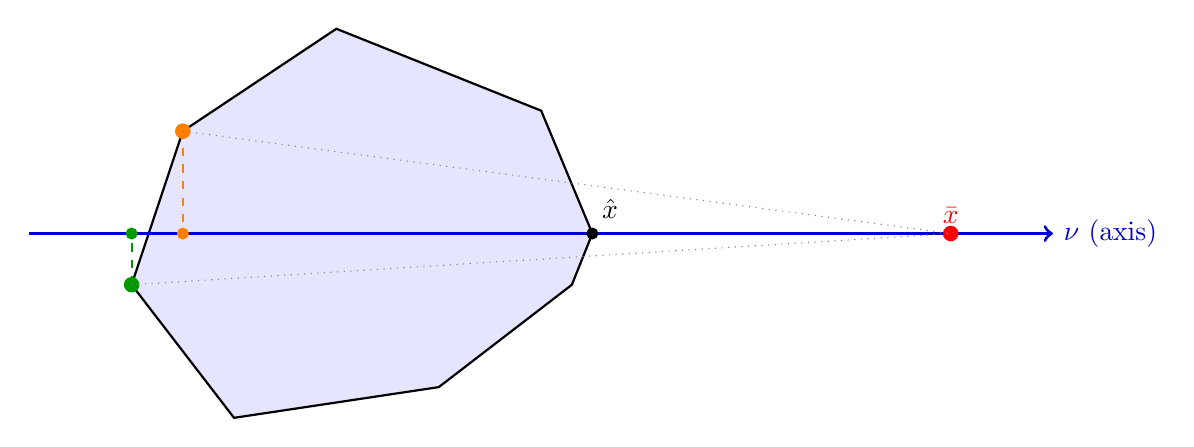
\begin{tikzpicture}[scale=1.3]
    \coordinate (xbar) at (5.5, 0);
    \coordinate (xhat) at (2.0, 0); 
    
    \coordinate (v1) at (2.0, 0);    % xhat (closest point)
    \coordinate (v2) at (1.5, 1.2);
    \coordinate (v3) at (-0.5, 2.0); 
    \coordinate (v4) at (-2.0, 1.0); % A "wide" vertex (large y, moderate x)
    \coordinate (v5) at (-2.5, -0.5); % v_star: The Farthest (deepest x, moderate y)
    \coordinate (v6) at (-1.5, -1.8);
    \coordinate (v7) at (0.5, -1.5);
    \coordinate (v8) at (1.8, -0.5);

    \draw[thick, fill=blue!10] (v1) -- (v2) -- (v3) -- (v4) -- (v5) -- (v6) -- (v7) -- (v8) -- cycle;

    \draw[->, very thick, blue!80!black] (-3.5, 0) -- (6.5, 0) node[right] {$\nu$ (axis)};
    
    \filldraw[red] (xbar) circle (2pt) node[above] {$\bar{x}$};
    \filldraw[black] (xhat) circle (1.5pt) node[above right, yshift=2pt] {$\hat{x}$};

    \filldraw[orange] (v4) circle (2pt);
    \coordinate (p3) at (-2.0, 0); % Projection of v3
    \draw[dashed, orange, thick] (v4) -- (p3);
    \filldraw[orange] (p3) circle (1.5pt);
    
    \filldraw[green!60!black] (v5) circle (2pt);
    \coordinate (p5) at (-2.5, 0); % Projection of v5
    \draw[dashed, green!60!black, thick] (v5) -- (p5);
    \filldraw[green!60!black] (p5) circle (1.5pt);

    \draw[dotted, gray] (v4) -- (xbar);
    \draw[dotted, gray] (v5) -- (xbar);

\end{tikzpicture}
\caption{Geometric intuition of Lemma \ref{lem:farthest_exact} for large $L$}
\end{figure}

\begin{remark}
In the limit as $L \to \infty$, the required margin $D^2/2L \to 0$. Thus, for large separation, maximizing distance is equivalent to minimizing $\inner{\nu}{v}$.
\end{remark}
\subsection{Exit Face Characterization}



\begin{proposition}\label{prop:exit_exact}
Let $F_0$ be the exit face with active constraints $\mathcal{A}_0$. For the constraint $a_i$, let $\theta_i$ be 
\begin{equation}\label{eq:theta_i}
\theta_i = \frac{\inner{a_i}{\nu}}{\|a_i\|}.
\end{equation}
If $L \geq D/\epsilon$ for some $\epsilon > 0$, then all active constraints on the exit face satisfy:
\begin{equation}\label{eq:alignment_bound}
\theta_i > -\epsilon \quad \forall i \in \mathcal{A}_0.
\end{equation}
\end{proposition}

\begin{proof}
Since $v^\star$ is good, the ray $r(t)$ travels through the interior of $\mathcal{P}$ for small $t > 0$ before terminating at the boundary point $x_{\text{exit}}$. By definition $x_{\text{exit}}$ lies in the relative interior of a unique face $F_0$. Now observe that $\forall i \in \mathcal{A}_0$, the function $t \mapsto a_i^\top r(t) = a_i^\top v^\star + t  a_i^\top(\bar{x} - v^\star)$ is strictly increasing implying $a_i^\top(\bar{x} - v^\star) > 0$.
Rewriting
\begin{equation*}
\bar{x} - v^\star = (\hat{x} + L\nu) - v^\star = L\nu + (\hat{x} - v^\star).
\end{equation*}
Substituting this into the inequality:
\begin{equation*}
L \inner{a_i}{\nu} + \inner{a_i}{\hat{x} - v^\star} > 0 \implies \inner{a_i}{\nu} > -\frac{\inner{a_i}{\hat{x} - v^\star}}{L}.
\end{equation*}
By Cauchy-Schwarz, $|\inner{a_i}{\hat{x} - v^\star}| \leq \|a_i\| \|\hat{x} - v^\star\| \leq \|a_i\| D$. Thus:
\begin{equation*}
\inner{a_i}{\nu} > -\frac{\|a_i\| D}{L}.
\end{equation*}
Dividing by $\|a_i\|$, and imposing $L \geq D/\epsilon$ yields $\theta_i > -\epsilon$.
\end{proof}

From Definition~\ref{def:adjacent}, one could interpret adjaceny in the following manner, for a polytope $\mathcal P$, faces $F_1, F_2$ are adjacent if and only if
$N_{\mathcal P}(F_1)$ and $N_{\mathcal P}(F_2)$ share a facet.
The following result, is the last technical statement needed before putting things together and relies on this interpretation. We make explicit that the preceding assumptions and definitions hold, that is, $\hat{x} \in \relint(F^\star)$ is the $M$-projection of $\bar{x}$ onto $\mathcal{P}$, and
$\nu$ the associated outward normal.
We assume $N_{\mathcal{P}}(\hat{x})$ has non-empty interior. Finally we denote $v^\star$ as the farthest good vertex.

\begin{lemma}\label{lem:exit_close}
There exists $L_0 > 0$ such that, for all
$L = \|\bar{x} - \hat{x}\| \ge L_0$, the face $F_0$ is either $F^\star$ or adjacent to $F^\star$.
\end{lemma}
\begin{proof}
We proceed in several steps. For a polytope $P$, the collection of normal cones
\[
\mathcal{N}(P) := \{ N_P(F) : F \text{ a face of } P \}
\]
forms a complete polyhedral fan in $\mathbb{R}^n$.
In particular: ($i$) each $N_P(F)$ is a closed polyhedral cone.
($ii$) The interiors of distinct normal cones are disjoint.
($iii$) If two faces $F_1$ and $F_2$ are adjacent, then
$N_P(F_1)$ and $N_P(F_2)$ share a common facet.
Conversely, if two normal cones share a facet, the corresponding faces are adjacent.
By assumption, $\nu \in \operatorname{int} N_P(F^\star)$.
Since $N_P(F^\star)$ is a polyhedral cone with nonempty interior,
there exists an open neighborhood $U \subset \mathbb{R}^n$ of $\nu$
such that
\[
U \subset \operatorname{int} N_P(F^\star).
\]
Because the normal cones form a polyhedral fan, the boundary
$\partial N_P(F^\star)$ consists of finitely many facets,
each shared with the normal cone of a face adjacent to $F^\star$.
Therefore, any vector sufficiently close to $\nu$ lies either in
$\operatorname{int} N_P(F^\star)$
or in the interior of a normal cone corresponding to a face adjacent to $F^\star$.
Write
$
d = \bar x - v^\star
= L\nu + (\hat x - v^\star).
$
So that,
\[
\frac{d}{\|d\|}
= \frac{L\nu + (\hat x - v^\star)}{\|L\nu + (\hat x - v^\star)\|}.
\]
Since $P$ is bounded, $\| \hat x - v^\star \| \le \operatorname{diam}(P)$.
Therefore,
\[
\frac{d}{\|d\|} \to \nu
\quad \text{as } L \to \infty.
\]
Consequently, there exists $L_0 > 0$ such that for all
$L \ge L_0$,
\[
\frac{d}{\|d\|} \in U.
\]
By construction of the ray and the exit point,
the direction $d$ belongs to the normal cone of the exit face:
$
d \in N_P(F_0).
$
Hence,
$
\frac{d}{\|d\|} \in N_P(F_0).
$
For $L \ge L_0$, we have $\frac{d}{\|d\|} \in U$,
which implies that
$\frac{d}{\|d\|}$ lies either in
$\operatorname{int} N_P(F^\star)$
or in the interior of a normal cone corresponding to a face adjacent to $F^\star$. Since interiors of normal cones are disjoint,  it follows that $F_0$ must be either $F^\star$
or a face adjacent to $F^\star$.
\end{proof}

\noindent With all the ingredients in place, we are now in position to provide a proof for Theorem~\ref{thm:main}.
\begin{proof}[Proof of Theorem~\ref{thm:main}]
Setting $L_0 = w_{\mathcal P}(\nu)$, the claim follows directly from Lemma~\ref{lem:farthest_exact}, Proposition~\ref{prop:exit_exact} and Lemma~\ref{lem:exit_close}.
\end{proof}

\subsection{Special Polytopes}


The result in Theorem~\ref{thm:main} and its associated analysis is very conservative (depending on the polytope diameter). Fortunately, for a the large class of well-conditioned polytopes in Definition~\ref{def:well_behaved}, this bound can be relaxed, and even dropped for a smaller subset. 

\begin{corollary}
\label{cor:exit_well_conditioned}
Assume $\mathcal P$ is $\kappa$-well-conditioned.
Let $F_0$ be the exit face with active constraints $\mathcal A_0$, and let $\theta_i$ as in~\ref{eq:theta_i}. If $L \;\ge\; \frac{\kappa}{\epsilon},$ 
then all active constraints on the exit face satisfy
$
\theta_i > -\epsilon
\quad \forall i \in \mathcal A_0.
$
\end{corollary}
\begin{proof}
By definition of the directional width,
\[
\min_{x \in \mathcal P} \langle \nu, x \rangle
\;\le\;
\langle \nu, v \rangle
\;\le\;
\max_{x \in \mathcal P} \langle \nu, x \rangle.
\]
Since $\hat x \in \mathcal P$, subtracting $\langle \nu, \hat x \rangle$
from all terms yields
\[
-\;w_{\mathcal P}(\nu)
\;\le\;
\langle \nu, v - \hat x \rangle
\;\le\;
w_{\mathcal P}(\nu),
\]
Applying Cauchy--Schwarz and Proposition~\ref{prop:exit_exact}
\begin{align*}
\bigl|\langle a_i, \hat x - v^\star \rangle\bigr|
&\;\le\;
\|a_i\| \, \bigl|\langle \nu, \hat x - v^\star \rangle\bigr|
\;\le\;
\|a_i\| \, w_{\mathcal P}(\nu)
\;\le\;
\|a_i\| \, \kappa \\
&\implies \langle a_i, \nu \rangle > -\frac{\kappa}{L} \|a_i\|.
\end{align*}
Imposing $L \ge \kappa/\epsilon$ concludes the proof.
\end{proof}



Below is an exact characterization of the preceding arguments for axis-aligned boxes (and their affine images), which are of special interest in systems and control. 
\begin{definition}
A box polytope is a set of the form
\[
\mathcal P = \{x \in \mathbb R^n : \ell \le x \le u\},
\]
with $\ell_i < u_i$ for all $i$.
\end{definition}
\begin{proposition}
\label{prop:box_no_threshold}
Let $\mathcal P = \{x \in \mathbb R^n : \ell \le x \le u\}$ be a box polytope,
let $\bar x \notin \mathcal P$, Then the farthest good vertex satisfies
\[
v^\star = \argmin_{v \in V_{\emph{good}}} \langle \nu, v \rangle
\quad \text{for all } L > 0.
\]
\end{proposition}
\begin{proof}
Vertices of $\mathcal P$ are of the form
\[
v(s)_i =
\begin{cases}
\ell_i & s_i = -1, \\
u_i & s_i = +1,
\end{cases}
\qquad s \in \{-1,+1\}^n.
\]
A vertex $v(s)$ is good if and only if $(\bar x_i - v_i(s)) s_i > 0 \quad \forall i,$
which fixes the sign $s_i$ uniquely for each coordinate.
The squared distance decomposes coordinate-wise:
\[
\|v(s) - \bar x\|^2
= \sum_{i=1}^n (\bar x_i - v_i(s))^2.
\]
For each coordinate $i$, among the two possible choices
$v_i \in \{\ell_i, u_i\}$, the good vertex selects the value farther from
$\bar x_i$. Hence the farthest good vertex is obtained by independently
maximizing each coordinate contribution. On the other hand,
\[
\langle \nu, v(s) \rangle
= \sum_{i=1}^n \nu_i v_i(s),
\]
which is minimized by the same coordinate-wise choice:
$v_i = \ell_i$ if $\nu_i > 0$ and $v_i = u_i$ if $\nu_i < 0$. Therefore the vertex minimizing $\langle \nu, v\rangle$
coincides exactly with the farthest good vertex, independently of $L$.
\end{proof}
